\Chapter{Nim játék, és Northcott-sakk példaprogram}

\section{Felhasználói dokumentáció}
\subsection{Rendszerkövetelmények}
A program Java-ban íródott, éppen ezért futtatásához Java SE 1.8 futtatókörnyezet szükséges. A program nem támaszt különösebb rendszerkövetelményt a futtató géppel szemben, egy mai asztali számítógépen probléma nélkül el kell, hogy fusson. Legalább egy 1024x768-as felbontású monitor szükséges az ablak megjelenítéséhez, továbbá a programot egérrel, és billentyűzettel (vagy ezt kiváltó perifériákkal) lehet vezérelni.

\subsection{Telepítési útmutató}
A programot nem szükséges telepíteni, a Java archívumot (.jar) egyszerűen a Java futtatókörnyezetével elindítva a program futtatható. A szoftver nem igényel különösebb rendszerjogosultságokat.

\subsection{A program használata}
A programot elindítva az \myref{fig:fokepernyo} főképernyő fogad minket:\\
\begin{figure}[h]
	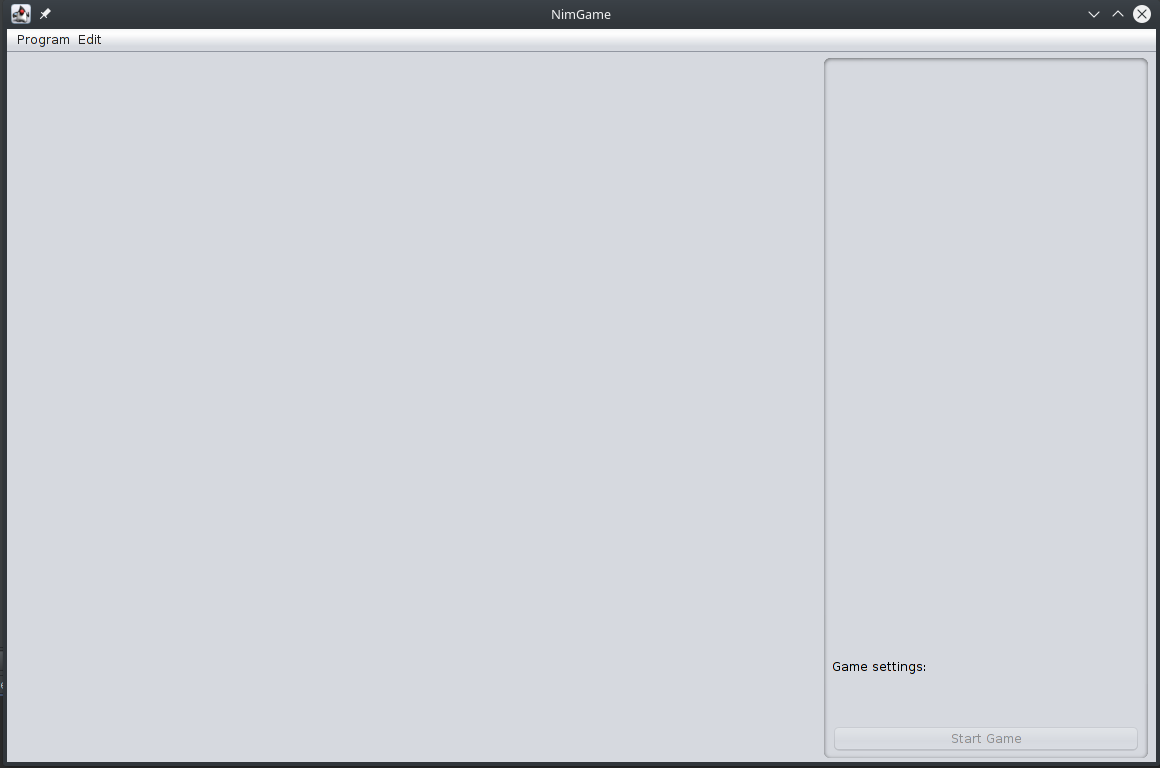
\includegraphics[width=10cm, height=8cm]{program/fokepernyo}
	\centering
	\caption{A példaprogram főképernyője}
	\label{fig:fokepernyo}
\end{figure}

A szoftver úgy lett megtervezve, hogy több különböző (nem feltétlenül csak Nim) játék futtatására legyen alkalmas, de alapvetően mindegyik játék három főbb elemmel rendelkezik. A beállításpanellel, az állapotpanellel, és a főpanellel. Az első kettő a jobb oldalon található oldalsó panelen jelenik meg, míg a főpanel az ablak nagyobb részét kitöltő üres helyen helyezkedik el, amint a megfelelő játékot betöltjük. \\

Játékot betölteni a "Program" menü (\myref{fig:program_menu}) "Select game" almenü segítségével lehet megtenni. Itt ki kell választani a kívánt játékot. 
\begin{figure}[h]
	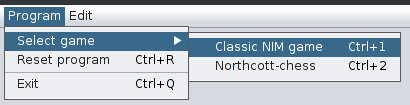
\includegraphics[width=8cm, height=2cm]{program/program_menu}
	\centering
	\caption{A főképernyő program menüje}
	\label{fig:program_menu}
\end{figure}


Jelenleg két játék közül lehet választani, ezeknek a leírására külön szekciót szentelek. Az aktuális játékot bezárni a "Reset program" menüelemmel lehetséges, továbbá a programból kilépni az "Exit" menüelemmel használatával tud a felhasználó.\\

Ezek a menüelemek a program futása során bármikor elérhetőek, azonban fontos megjegyezni, hogy amennyiben futó játék alatt egy másik játéktípus kerül kiválasztásra, abban az esetben az éppen játszott játék bezárásra kerül csak úgy, mintha a "Reset program" menüelemet választottuk volna.\\

A legtöbb menüelemet gyorsbillentyű segítségével is aktiválni lehet. Hogy melyik elemhez milyen gyorsbillentyű tartozik arról a menüfelirat mellett elhelyezkedő billentyűparancs ad tájékoztatást.

\subsection{Klasszikus Nim Játék}
A klasszikus Nim - mint arra a neve is utal - a hagyományos Nim játék megvalósítása. Az \myref{fig:nim_ingame} ábra éppen azt mutatja, amint a gép ellen játszok. Jól látszik, hogy a játékban (éppen) 4 halom van, amelyekben a kavicsok darabszáma rendre 7, 9, 8, 7. Az állapotablakban jól látszik, hogy négy körön már túl is vagyunk.
\begin{figure}[h]
	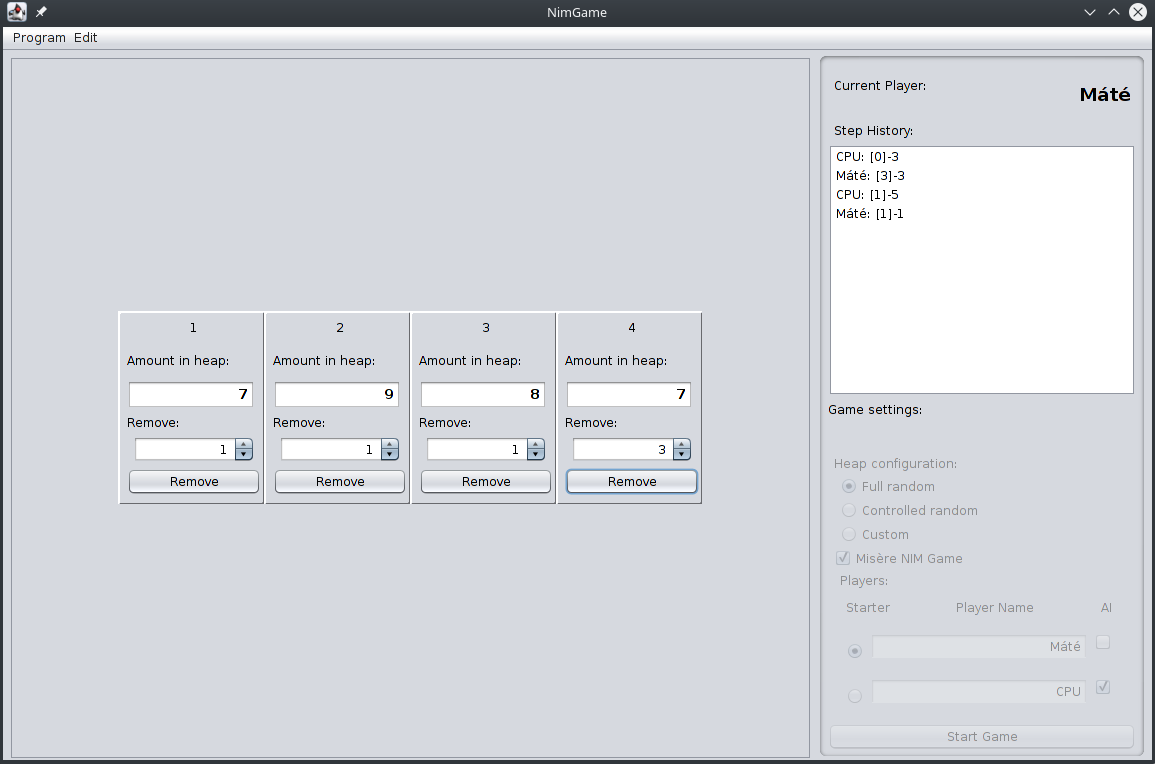
\includegraphics[width=14cm, height=10cm]{program/nim_ingame}
	\centering
	\caption{Klasszikus Nim játék a gép ellen}
	\label{fig:nim_ingame}
\end{figure}

A játék kezdete előtt lehetőségünk van részletekbe menően beállítani, hogy pontosan hogyan szeretnénk játszani a játékot. Ehhez be kell állítanunk a halom konfigurációt, és a játékosokat. Miután a beállításokkal végeztünk az oldalsó panel alján található "Start Game" gombbal kezdhetjük a játékot. Ez után a beállítások módosítása már nem lehetséges, de bármikor kezdhető új játék a már említett menüelemek használatával.

\subsubsection{Játékos beállítások}
A Nim-játék természetéből fakadóan két "személy" játssza. A szövegbeviteli mezőkbe a játékosok neveit kell megadni (eltérőeknek kell lenniük). A bal oldalon található rádiógomb segítségével azt választhatjuk ki, hogy ki kezdjen, még a jobb oldalon elhelyezkedő jelölőnégyzet arra szolgál, hogy tudassuk a programmal, hogy azt a játékost ő vezérli.\\
A beállítások adta szabadságból látszik, hogy a programmal lehet ember-ember, gép-ember, és gép-gép játékot is játszani.

\subsubsection{Halom beállítások}
A halombeállítások kezdetén azt kell eldönteni, hogy milyen mélységben szeretnénk beleszólni a kezdeti játéktér felépítésébe. Ezt vezérelni a "Heap Configuration" szöveg alatti rádiógomb-csoporttal lehetséges. Ezekre kattintva a felület dinamikusan átalakul további funkciókat felfedve. 

\begin{itemize}
	\item Full random: Teljes egészében a programra bízzuk, hogy hány halmot generál milyen elemszámmal
	\item Controlled random: Továbbra is a gépre bízzuk, hogy összeállítsa a játékteret, azonban a generálás szabályokat ezzel vezérelni tudjuk. Erre kattintva a \myref{fig:nim_settings_controlledrandom} panel megjelenik, ahol az első sorban a halom számát, a második sorban a halmok elemszámára tudunk egyéni korlátot megadni. Az első oszlop az alsó korlátot, a második pedig a felső korlátot adja meg.
	\item Custom: Itt teljesen megszabjuk, hogy hány halmot szeretnénk milyen elemszámmal. Erre a gombra kattintva egy új panel (\myref{fig:nim_settings_custom}) jelenik meg, ami egy szövegbeviteli mezőből áll. A mezőbe szóközzel elválasztva kell megadni, hogy a halmokban hány elem legyen. Mindegyik szám egy halmot reprezentál, és a halmok az itt megadott sorrendben fognak létrejönni.
\end{itemize}

Amennyiben Misère Nim játék helyett normál módon akarunk játszani, akkor a "Misère NIM Game" jelölőnégyzetetek szüntessük meg a bejelöltségét.

\begin{figure}[h]
	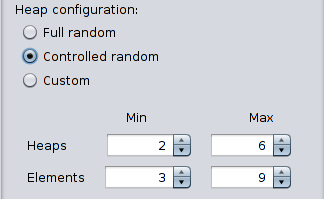
\includegraphics[width=5cm, height=3cm]{program/settings_controlled_random}
	\centering
	\caption{Irányított generálás}
	\label{fig:nim_settings_controlledrandom}
\end{figure}

\begin{figure}[h]
	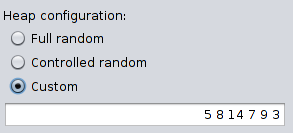
\includegraphics[width=5cm, height=2cm]{program/settings_custom}
	\centering
	\caption{Egyedi halomkonfiguráció}
	\label{fig:nim_settings_custom}
\end{figure}

\subsubsection{A játék menete}
Miután végeztünk a beállításokkal kattintsunk a "Start Game" gombra, és a játék elindul. Ekkor a jobb felső sarokban található állapotablak tájékoztat minket arról, hogy ki az éppen soron lévő játékos. \\

A főpanelon látszódnak a halmok 1-1 panel formájában. Mindegyik panel tetején megtalálható a panel sorszáma, alatta egy szövegbeviteli mezőben a halomban található elemek száma, az alatt egy pörgettyűben beállítható az elvenni kívánt elemek darabszáma, majd legalul az elvesz gomb. \\

Az éppen soron következő játékosnak meg kell hoznia megfelelő döntést, és lépnie kell oly módon, hogy a kiválasztott halomhoz tartozó pörgettyűbe beállítja mennyivel szeretné csökkenteni a halom elemszámát, és megnyomja a halomhoz tartozó "Remove" gombot. Ekkor a halom elemszáma csökken, a játékos köre véget ér, és a következő játékos kerül sorra. Amennyiben egy halom elfogy abban az esetben az azt reprezentáló panel eltűnik.\\

A játék véget ér, amennyiben mindegyik halom elfogy, és a program egy előugró üzenetben ad tájékoztatást arról, hogy melyik játékos nyerte meg a játékot.

\subsection{Northcott-sakk}
\subsubsection*{A játék beállítása}
A Northcott-sokk sok tekintetben hasonlít a hagyományos Nim játékra, éppen ezért beállítása is hasonlóan történik. A szövegbeviteli mezőkbe a játékosnevet kell írni, a bal oldali rádiógomb kiválasztja a kezdőjátékost, míg a jobb kéz felől található jelölőnégyzet a játékost gépinek jelöli.\\

Ami viszont lényeges eltérés, hogy itt a halom beállításai mások, mint a Nim esetében. A \myref{fig:northcott-settings} ábrát megfigyelve lényegesen leszűkültek a beállítási lehetőségek. Itt gyakorlatilag csak a sakktábla dimenzióját adhatjuk meg. A "Horizontal" (Vízszintes) az oszlopok számát, míg a "Vertical" (függőleges) a sorok számát adja meg. Ez nim játékra levetítve oszlop darab halom, és minden halomban maximálisan sor darab elem.

\begin{figure}[h]
	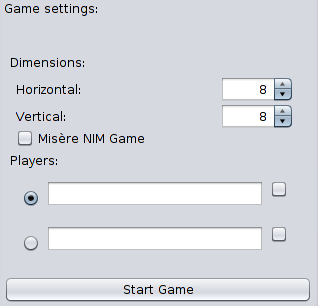
\includegraphics[width=5cm, height=5cm]{program/northcott-settings}
	\centering
	\caption{Northcott-sakk beállítópanelje}
	\label{fig:northcott-settings}
\end{figure}

Ez a játék is játszható Misère módon, a hozzá tartozó "Misère NIM Game" jelölőnégyzettel lehet állítani, hogy Misère, vagy normál módon kívánunk játszani.

Látható, hogy a véletlen halomgenerálás teljesen eltűnt. Ennek az az oka, hogy a játék kezdése előtt van egy extra művelet, ami nem teszi lehetségessé a véletlen generálást.

\subsubsection*{A játék előkészítése}
Ha végeztünk a játékbeállításokkal, akkor még ne indítsuk el a játékot, ugyanis a játékosoknak lehetőségük van beállítani a bábujuk kezdő pozícióját. A játéktér kezdetben minkét játékos térfelét elfedi. A térfeleket az főpanel alján lévő két vezérlőgombbal lehet fel, illetve elfedni. A gép által vezérelt játékos bábuinak kezdőpozíciója nem állítható, így a hozzá tartozó gomb eltávolításra kerül, ha jelölőnégyzet bejelölésre kerül.\\

\begin{figure}[h]
	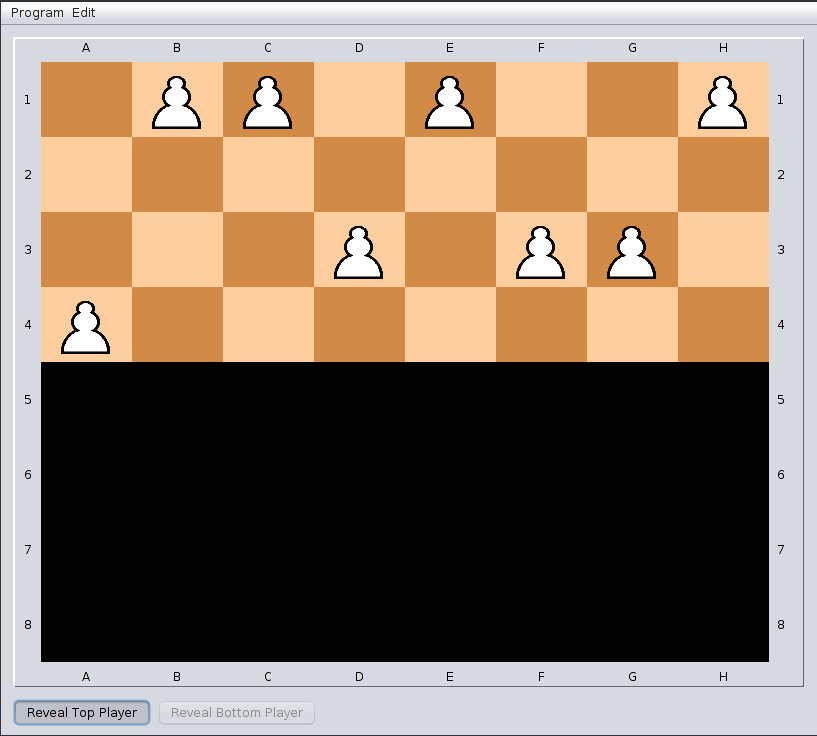
\includegraphics[width=8cm, height=8cm]{program/northcott-setup}
	\centering
	\caption{Northcott-sakk kezdő pozíciók beállítása}
	\label{fig:northcott-setup}
\end{figure}

A felső játékos - miután meggyőződött arról, hogy ellenfele nem figyeli - a "Reveal Top Player" gombra kattintva felfedi saját játékterét. Felfedett állapotba a gomb "beragad", és a másik gomb letiltódik, hogy véletlenül ne lehessen az ellenfél térfelére átváltani. A felső játékos a kívánt mezőre kattintva áthelyezheti az adott oszlopban lévő bábuját arra a mezőre, amelyikre kattintott. Ha a felső játékos késznek érzi a kezdőállapotot, akkor a beragadt gombra újból rákattintva elfedi a felső játékteret, és átadja a helyét az alsó játékosnak, aki ugyan ezt a műveletsort végigjátssza. \\

Miután mindketten végeztek a beállítással a játék a "Start Game" gombra kattintva indítható. Ez után a játék beállításai már nem módosíthatóak, a beállításoz tartozó vezérlőelemek letiltásra, a játéktér elrejtéséért/felfedéséért felelős vezérlőgombok eltávolításra kerülnek.


\subsubsection*{A játék menete}
A játék indulásakor a teljes játéktér felfedésre kerül, és a program a jobb felső sarokban található állapotpanelen tájékoztat a soron következő játékos kilétéről. Lépni úgy lehet, hogy a kiválasztott oszlopban arra a mezőre kattintunk, ahova a saját bábunkkal lépni szeretnénk. A mezőre kattintva a lépés bekövetkezik, és a játékos köre véget ér, helyére a következő játékos lép.\\

\begin{figure}[h!]
	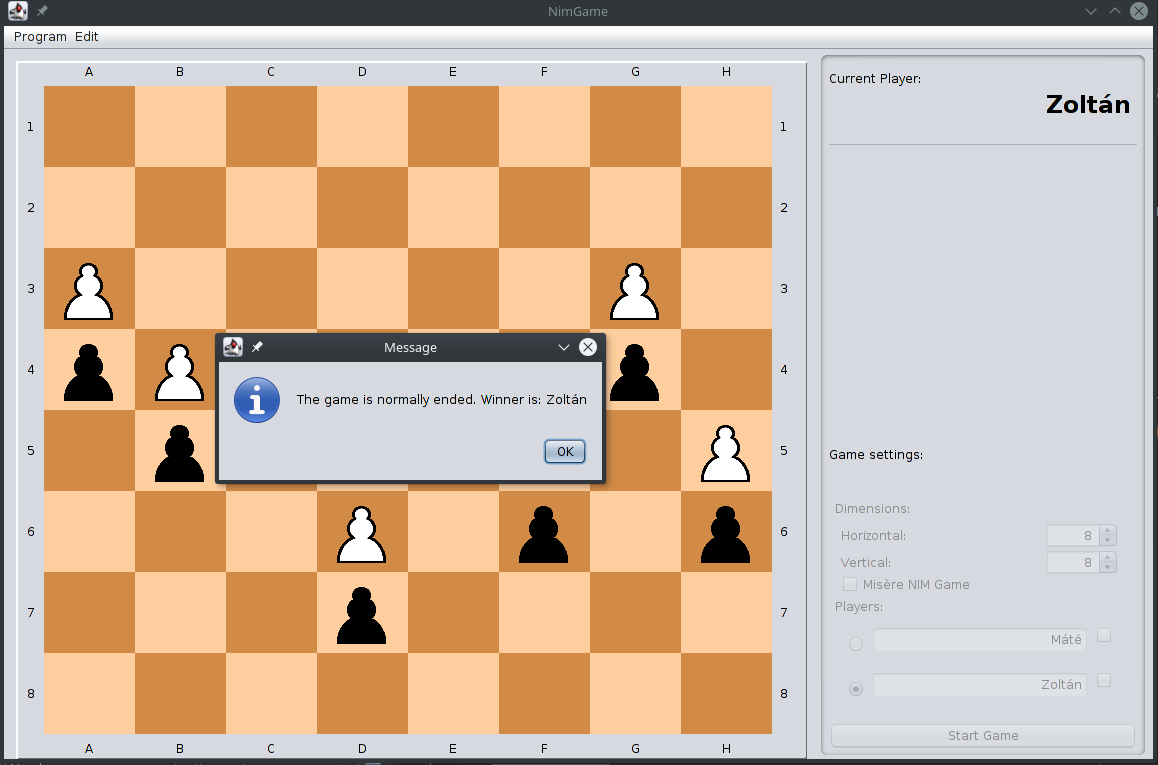
\includegraphics[width=12cm, height=8cm]{program/northcott-end}
	\centering
	\caption{Northcott-sakk játék vége; nyertes játékos Zoltán}
	\label{fig:northcott-end}
\end{figure}

A játék addig tart, amíg van olyan oszlop, ahol a bábuk között lévő távolság nagyobb, mint 0, azaz nem közvetlenül egymás mellett áll mindegyik bábu. A játék végén a program egy előugró ablakban ad tájékoztatást arról, hogy a játékot melyik játékos nyerte meg.


\section{Fejlesztői dokumentáció}

Nem célom a teljes forráskód beillesztése a dolgozatba, mert egyrészt viszonylag nagy méretű, (több ezer sor) sok rész triviális, vagy csak technikai, azonban bizonyos osztályokat, vagy kódrészleteket behivatkozok, amikben úgy érzem, hogy említésre méltó dolgok találhatóak.

\section{Nim nyerő stratégia gépi implementációja}
A gépi játékost stratégiáját a AINimWinningStrategy osztály valósítja meg, amely implementálja a NimAI interfészt:
\lstinputlisting[language=java]{source/nimgame/core/AI/NimAI.java}

A visszaadott NimAISolution objektum gyakorlatilag egy tárolóobjektum amely a kiválasztott halmot, és az abból elvett elemszámot tartalmazza.

Maga a stratégia implementációja jól követi az elméleti részben tárgyalt stratégiát, de néhány helyen magyarázatot igényel. \\
A belépési pont a getNextStep() metódus, ami paraméterben megkapja a halomlistát. Ezután ezt átalakítja tömbbé, és meghívja a getBestMove() metódust. Az átalakítás nem szükséges, de az adatstruktúrán igen sok műveletet hajt végre az algoritmus, így optimálisabb ezzel az átalakítással.\\
A getBestMove() a gerince a stratégiának, itt dől el, hogy a mesterséges intelligencia melyik lépést választja a következőnek. Először is megkeresi az első nem üres halmazt, (ha mindegyik halmaz üres, akkor dobunk egy kivételt, az MI nem futtatható üres játéktéren) majd egyszerű próbálkozással nekiáll megkeresni az első olyan állapotot, amit a decisionMaker elfogad. Minden halomra (ha nem üres) megpróbálja elfogadtatni az lépést úgy, hogy először elvesz az aktuális halomból egyet, majd kettőt, és így tovább amíg el nem fogy a halom. Ha az egész halmot elvette, de még mindig nem fogadta el a lépést a DecisionMaker, akkor visszaállítja a halom elemszámát a kísérletezés előtti állapotra, és lép a következő halomra.\\
A DecisionMaker egy belső interfész, melyet két belső osztály implementál. Feladata az, hogy eldöntse, hogy az éppen vizsgált lépés elfogadható-e legjobb lépésnek. Az a két belső osztály ami implementálja az pont a NimStandardDecisionMaker, és a NimMisereDecisionMaker. Mint a nevükből kiderül az egyik a hagyományos Nim játéknál hoz döntést, míg a másik a Misère módhoz. Első megközelítésben nem sok értelme látszik ennek a fajta megoldásnak, hiszen ezt a vizsgálatot beleépíthettem volna a kereső algoritmusba, azonban ha így tettem volna, akkor minden ciklusfutáskor kellett volna tennem egy feltételvizsgálatot, hogy éppen melyik módban van a játék. Így azonban a konstruktorban elvégzem ezt a vizsgálatot, és a mezőhöz a megfelelő DecisionMaker objektumot rendelem hozzá, így a ciklusban az összes ilyen vizsgálat elhagyható tovább gyorsítva az algoritmust.\\
Ez az algoritmus majdnem minden esetben talál nyerő állapotot, kivéve, ha az ellenfél kezdett, és hibátlanul játszik. Ebben az esetben nem tud mit csinálni, így - mivel nincs jó megoldás, de lépni kell - elvesz az első nem üres halomból halomból egyet.

\lstinputlisting[language=java]{source/nimgame/core/AI/AINimWinningStrategy.java}

